\section{Calibration using a photometric correction {\color{blue} Laurence} }
\label{se:photocorr_calibration}

As discussed in Sect.~\ref{se:obsdate_variations}, observations during the
afternoon sessions or
%the morning session after observations close to the direction of the
%Sun
during sunrise
are deeply affected by the telescope-driven beam
size variations, which are either due to an increase of the main dish
temperature (afternoons) or to a focus drift (sunrises).
For the baseline calibration presented in
Sect.~\ref{se:baseline_calibration}, this effect was mitigated by
discarding the scans acquired during these periods, as defined by the
baseline selection of Sect.~\ref{se:data_selection}. However, in
this section, we address the issue of calibrating in
telescope-driven unstable observing conditions. We discuss a
calibration method that relies on a photometric correction
depending on the beam size. 

When using the photometric correction, no scan selection based on the
observation date is performed. However, the scans from which the
absolute calibration is derived, are selected on the FWHM estimate
using the same criteria as for the baseline calibration. Thus, only
the scans that are moderately affected by the beam effect are included
in the absolute calibration in order not to include twice the
photometric correction uncertainties in the error budget (once for the
absolute calibration and once for the photometry).

We perform two case studies: Sect.~\ref{se:photocorr_demo} presents a demonstration
calibration assuming the beam is precisely monitored, whereas
Sect.~\ref{se:photocorr_pointing} addresses a practical calibration relying
on a beam monitoring using pointing scans. 


\subsection{Photometric correction methods}
\label{se:photocorr_methods}




\subsection{Demonstration case}
\label{se:photocorr_demo}

\addparag{ demo case}

Fig.~\ref{fig:calib_uranus_vs_atmtrans_all} shows the
measured-to-expected flux density ratio of Uranus observations after
calibrating using the demonstration case of the beam-variation
hardened calibration. 


\subsection{Practical case using pointing scans}
\label{se:photocorr_pointing}

\addparag{ pointing-based photometric correction}

Fig.~\ref{fig:calib_uranus_vs_atmtrans_all} shows the
measured-to-expected flux density ratio of Uranus observations after
calibrating using the practical case of the beam-variation
hardened calibration. 

\begin{figure}[ht!]
\begin{center}
  % corrected skydip
    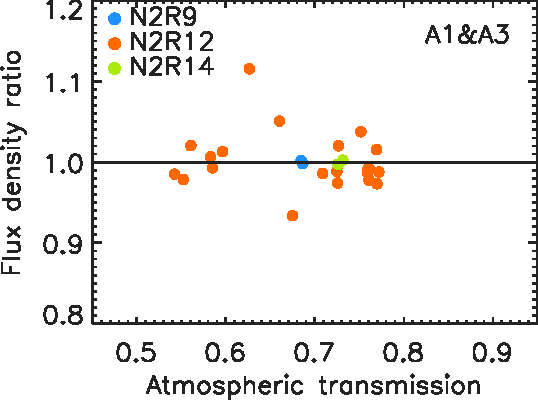
\includegraphics[clip=true, trim={0, -0.3cm, -0.3cm, 0}, width=0.35\textwidth]{Figures/Calibration/plot_flux_density_ratio_obstau_uranus_corrected_skydip_narrow_1mm.pdf}\hspace{0.2cm}
    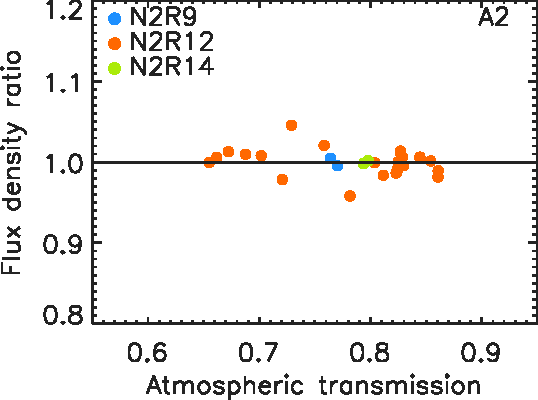
\includegraphics[clip=true, trim={0, -0.3cm, -0.3cm, 0}, width=0.35\textwidth]{Figures/Calibration/plot_flux_density_ratio_obstau_uranus_corrected_skydip_narrow_a2.pdf}
    \vspace{0.3cm}
    % taumeter
    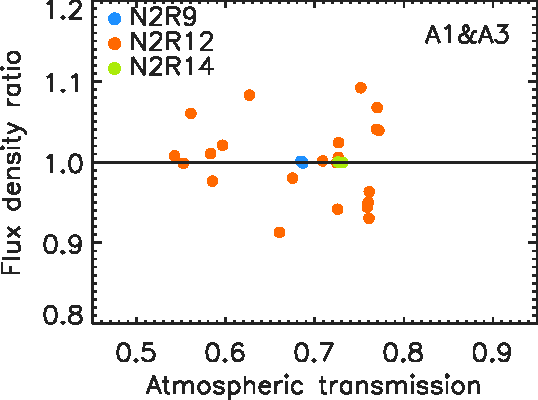
\includegraphics[clip=true, trim={0, -0.3cm, -0.3cm, 0}, width=0.35\textwidth]{Figures/Calibration/plot_flux_density_ratio_obstau_uranus_tau225_narrow_1mm.pdf}\hspace{0.2cm}
    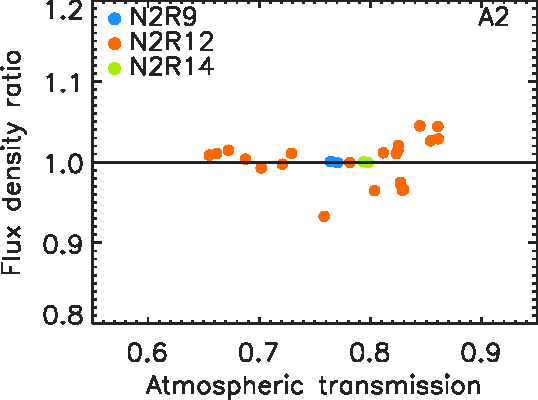
\includegraphics[clip=true, trim={0, -0.3cm, -0.3cm, 0}, width=0.35\textwidth]{Figures/Calibration/plot_flux_density_ratio_obstau_uranus_tau225_narrow_a2.pdf}
    \vspace{0.3cm}
    % skydip
    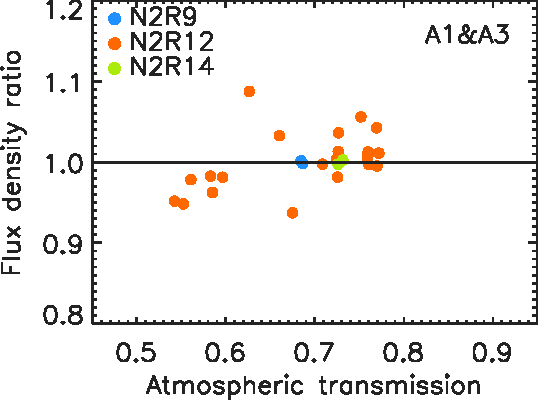
\includegraphics[clip=true, trim={0, -0.3cm, -0.3cm, 0}, width=0.35\textwidth]{Figures/Calibration/plot_flux_density_ratio_obstau_uranus_skydip_narrow_1mm.pdf}\hspace{0.2cm}
    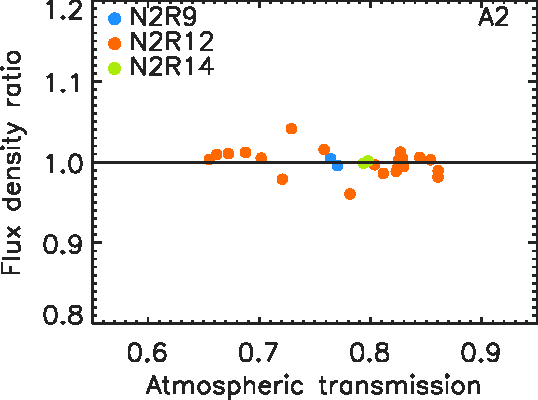
\includegraphics[clip=true, trim={0, -0.3cm, -0.3cm, 0}, width=0.35\textwidth]{Figures/Calibration/plot_flux_density_ratio_obstau_uranus_skydip_narrow_a2.pdf}
    \vspace{0.3cm}
    % corr. sky. photocorr demo
    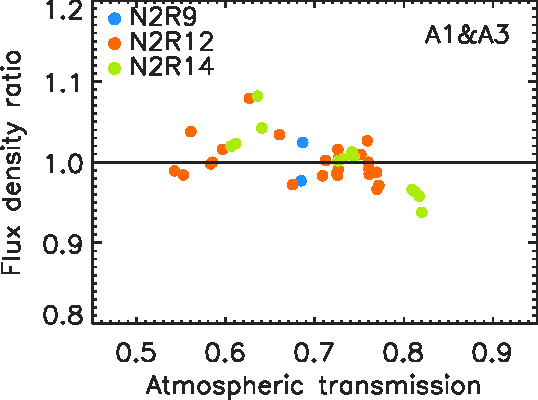
\includegraphics[clip=true, trim={0, -0.3cm, -0.3cm, 0}, width=0.35\textwidth]{Figures/Calibration/plot_flux_density_ratio_obstau_uranus_corrected_skydip_photocorr_demo_narrow_1mm.pdf}\hspace{0.2cm}
    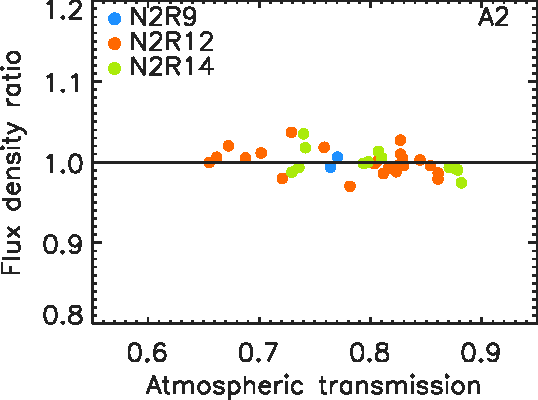
\includegraphics[clip=true, trim={0, -0.3cm, -0.3cm, 0}, width=0.35\textwidth]{Figures/Calibration/plot_flux_density_ratio_obstau_uranus_corrected_skydip_photocorr_demo_narrow_a2.pdf}
    \vspace{0.3cm}
    % corr. sky. photocorr pointing
    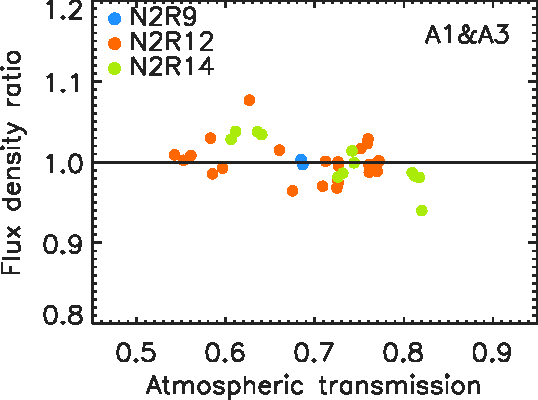
\includegraphics[clip=true, width=0.35\textwidth]{Figures/Calibration/plot_flux_density_ratio_obstau_uranus_corrected_skydip_photocorr_pointing_narrow_1mm.pdf}\hspace{0.2cm}
    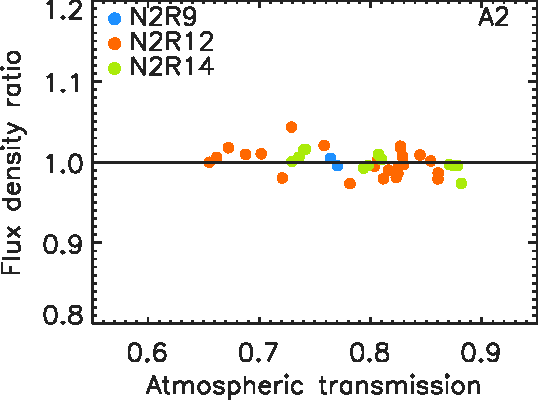
\includegraphics[clip=true, width=0.3337\textwidth]{Figures/Calibration/plot_flux_density_ratio_obstau_uranus_corrected_skydip_photocorr_pointing_narrow_a2.pdf}
\caption[Uranus flux density stability using the
  practical case of the beam-hardened calibration]{For the
  practical case of the beam-hardened calibration, 
  ratio of the Uranus measured flux densities to expectations as a
  fonction of the measured 2D Gaussian beam FWHM (top) and as a
  function of the observed opacity (bottom) for the 1mm array
  combination (left) and for array 2 (right),
  including scans acquired during N2R9, N2R12 and N2R14 campaigns. }
\label{fig:calib_uranus_vs_atmtrans_all}
\end{center}
\end{figure}



% ALL METHOD RESULTS 
\begin{table}[th]
\begin{center}
\begin{tabular}{|c|l|c|c|c|c|c|}
  \hline
  \multicolumn{2}{|c|}{}  &  \multicolumn{5}{|c|}{Methods} \\\cline{3-7}
  \multicolumn{2}{|c|}{Characteristics} &  baseline  & taumeter  &  skydip  &  photocorr demo & photocorr pointing \\
  \hline\hline
   \multicolumn{2}{|c|}{$\#$ selected scans} & 26    &       26  &    26    &    38           &    38 \\ 
  \hline 
  Factor &  A1          &   1.00  &  0.97   &  1.13    &   1.02    &   1.01  \\
       &  A3            &   1.00  &  0.97   &  1.02    &   1.02    &   1.00  \\
       &  1mm           &   1.00  &  0.95   &  1.06    &   1.02    &   1.01  \\
       &  2mm           &   1.00  &  0.94   &  0.99    &   1.03    &   1.02  \\
  \hline
  RMS  &  A1            &  3.1    &   4.2   &   3.4    &    3.0    &   2.8 \\
       &  A3            &  3.7    &   4.3   &   3.3    &    3.1    &   2.9 \\
       &  1mm           &  3.2    &   4.5   &   3.3    &    2.7    &   2.5 \\
       &  2mm           &  1.6    &   2.6   &   1.5    &    1.3    &   1.5 \\
\hline\hline
\end{tabular}
\caption[Comparison of calibration results using five methods]{Comparison of calibration results using five methods}
\label{tab:Abs_calibration_results_all}
\end{center}
\end{table}





